\documentclass[12pt]{article}

% fonts

\usepackage[T1]{fontenc}
\usepackage{newtxtext}
\usepackage{bm}
\usepackage{amsthm} % before newtxmath b/c latex
\usepackage{newtxmath}
% \usepackage[bb=boondox,cal=cm]{mathalpha}
\usepackage{cancel}
\usepackage{amsmath}
\usepackage{amsfonts}
\usepackage{thmtools}
\usepackage{mathtools}
\usepackage{mathrsfs}
\usepackage{hyperref}
\usepackage{wrapfig}
% spacing

\usepackage[parfill]{parskip}
\setlength{\parindent}{0pt}
\setlength{\parskip}{2ex plus 0.2ex minus 0.2ex}

% geometry of the page

\usepackage[
paper  = letterpaper,
left   = 1in,
right  = 1in,
top    = 1in,
bottom = 1in,
]{geometry}

% references

\usepackage{natbib}


\begin{document}

\begin{flushleft}
\textbf{PSET 2 APMA4302} \\
Fred Angelo Garcia (fbg2107) \\
\today
\end{flushleft}

\vspace{0.1in}

\section{Question 1 condition number of a matrix}
we are told is defined as 
\begin{equation}
    \kappa(A) = \|A\| \|A^{-1}\|
\end{equation}
where $A$ is an invertible matrix, whose norm $||A||$ has the property that $||A{\bf x}|| \leq ||A||~ ||{\bf x}||$.

Glancing at this definition, it sort of looks like the condition number is a measure of how much the matrix $A$ can stretch a vector ${\bf x}$. So that it can effectively measure how sensitive the output of a linear system is (e.g., in our case)
\begin{equation}
    A{\bf u} = {\bf b}
\end{equation}
to small errors in the input. Where 
\begin{itemize}
    \item $A$ is the matrix of coefficients,
    \item ${\bf u}$ \textit{exact} solution, and
    \item ${\bf b}$ is the exact right hand side.
\end{itemize}

When we solve it numerically, we get an \textit{approximate} solution $\hat{\bf u}$, along with the approximate right hand side $\hat{\bf b}$, which we can think of as being perturbations of the exact solution and right hand side, respectively. So we can write
\begin{equation}
    A\hat{\bf u} = \hat{\bf b}
\end{equation}
where the solution computed found $\hat{\bf u} = {\bf u} + \delta {\bf u}$ can be thought of as a perturbation of the exact solution ${\bf u}$, and $\hat{\bf b} = {\bf b} + \delta {\bf b}$ can be thought of as a perturbation of the exact right hand side ${\bf b}$.

The error in the solution is ${\bf u} - \hat{\bf u}$. 

\subsection{part (a)}

We can use the two systems to write the error in the solution as
\begin{equation}
    {\bf u} - \hat{\bf u} = A^{-1}{\bf b} - A^{-1}\hat{\bf b} = A^{-1}({\bf b} - \hat{\bf b})
\end{equation}
which expresses the solution in the error in terms of the error in the right hand side, and $A$ is again invertible. 

We can then take norms of both sides to get
\begin{equation}
    \|{\bf u} - \hat{\bf u}\| = \|A^{-1}({\bf b} - \hat{\bf b})\| 
\end{equation}
and, using the matrix norm property we state above, we can write
\begin{equation}
    \|{\bf u} - \hat{\bf u}\| \leq \|A^{-1}\| \|{\bf b} - \hat{\bf b}\|
    \label{eq:1}
\end{equation}
we can sugestively write ${\bf b} = A{\bf u}$ and take the norms, and use the norm property again to get lower bound on $\|{\bf u}\|$ as
\begin{equation}    
    \|{\bf b}\| = \|A{\bf u}\| \leq \|A\| \|{\bf u}\| \Rightarrow \|{\bf u}\| \geq \frac{\|{\bf b}\|}{\|A\|}.
    \label{eq:2}
\end{equation}
OK, then define the relative error in the solution as $\frac{\|{\bf u} - \hat{\bf u}\|}{\|{\bf u}\|}$. And, combinin Eqs \ref{eq:1} and \ref{eq:2}, we can write
\begin{equation}
    \frac{\|{\bf u} - \hat{\bf u}\|}{\|{\bf u}\|} \leq \|A^{-1}\| \|{\bf b} - \hat{\bf b}\| \frac{\|A\|}{\|{\bf b}\|}
\end{equation}
and recall the definition of the condition number $\kappa(A) = \|A\| \|A^{-1}\|$, we can write
\begin{equation}
    \frac{\|{\bf u} - \hat{\bf u}\|}{\|{\bf u}\|} \leq \kappa(A) \frac{\|{\bf b} - \hat{\bf b}\|}{\|{\bf b}\|}
\end{equation}
which shows that the relative error in the solution is less than or equal to the condition number times the relative error in the right hand side, as we wanted to show.    


\subsection{part (b)}
We are given two systems, $A {\bf u} = {\bf b}$ and $A {\bf e} = {\bf r}$, where thbe error in the solution ${\bf e = }{\bf u} - \hat{\bf u}$ and the residual ${\bf r} = {\bf b} - A\hat{\bf u}$. And we are to prove that 
\begin{equation}
\dfrac{1}{\kappa(A)} \dfrac{\|{\bf r}\|}{\|{\bf b}\|} \leq \dfrac{\|{\bf e}\|}{\|{\bf u}\|} \leq \kappa(A) \dfrac{\|{\bf r}\|}{\|{\bf b}\|}.
\end{equation}
Note, we can also use definition of the residual to write $A\hat{\bf u} = {\bf b} - {\bf r}$. 

We can use the statement form the book that the norm of the error is bounded by the norm of the residual as $\|{\bf e}\| \leq \|A^{-1}\| \|{\bf r}\|$. 

And we show above that $\| {\bf u} \| \geq \dfrac{\|{\bf b}\|}{\|A\|}$.

So that the upper bound becomes
\begin{equation}
\dfrac{\|{\bf e}\|}{\|{\bf u}\|} \leq \|A^{-1}\| \|{\bf r}\| \cdot \dfrac{\|A\| }{\|{\bf b}\|}  = \kappa(A) \dfrac{\|{\bf r}\|}{\|{\bf b}\|}
\end{equation}

The lower bound can be shown from ${\bf r } = A {\bf e}$.
\begin{equation}
    \|{\bf r}\| = \|A {\bf e}\| \leq \|A\| \|{\bf e}\| \Rightarrow \|{\bf e}\| \geq \dfrac{\|{\bf r}\|}{\|A\|}
\end{equation}

and $\frac{1}{\|{\bf b}\|} \leq \frac{1}{\|A\| \|{\bf u}\|}$, so that we can write
\begin{equation}
    \dfrac{\|{\bf e}\|}{\|{\bf u}\|} \geq \dfrac{\|{\bf r}\|}{\|A\| \|{\bf u}\|} \geq \dfrac{\|{\bf r}\|}{\|A\| \|A^{-1}\| \|{\bf b}\|} = \dfrac{1}{\kappa(A)} \dfrac{\|{\bf r}\|}{\|{\bf b}\|}
\end{equation}
from this, we have shown the lower bound, giving all together
\begin{equation}
\dfrac{1}{\kappa(A)} \dfrac{\|{\bf r}\|}{\|{\bf b}\|} \leq \dfrac{\|{\bf e}\|}{\|{\bf u}\|} \leq \kappa(A) \dfrac{\|{\bf r}\|}{\|{\bf b}\|} 
\end{equation}

This shows that the relative residual ($\frac{\|{\bf r}\|}{\|{\bf b}\|}$) differs from the relative error ($\frac{\|{\bf e}\|}{\|{\bf u}\|}$) by at most a factor of the condition number $\kappa(A)$ and that if the conditioning is large, a small relative residual may not correspond to small error, conditioning is kinda a big deal.

\section{Question 2, tridiag matrix}

A tridiagonal matrix $A = \dfrac{1}{h^2} {\rm tridiag}(-1, 2, -1)$
\begin{itemize}
    \item we hagve the diff eq $-u''(x) = f(x)$, for $x \in [0, 1]$, and $f(x) = 0$ otherwise.
    \item centered finite difference discretization of the second derivative $u''(x)$ on the interval $[0, 1]$ 
    \item homogeneous Dirichlet boundary conditions $u(0) = u(1) = 0$.
    \item $h = 1/m$ is the grid spacing, and $m$ is the number of interior grid points
    \item $A$ is an $(m-1) \times (m-1)$ matrix
\end{itemize}

so for $m=5$, $A$ looks something like
\begin{equation}
    A = \dfrac{1}{h^2} \begin{bmatrix}
    2 & -1 & 0 & 0 \\
    -1 & 2 & -1 & 0 \\
    0 & -1 & 2 & -1 \\
    0 & 0 & -1 & 2
    \end{bmatrix}
\end{equation}

\subsection{part (a)}
 show that the eigenvectors of A are given by ${\bf v}_j = \sin\left(j \pi x_i \right)$ where $x_i = ih$ for $i = 1, \ldots, m-1$.

First, from the boundary conditions: $u(0) = u(1) = 0$, we know $u_0 = u_m = 0$, such that the unknowns we want are  $u_1, u_2, \ldots, u_{m-1}$.

We use the centered finite differnce discretization of the second derivative, which gives us
\begin{equation}
    -u''(x_i) \approx -\dfrac{u_{i-1} - 2u_i + u_{i+1}}{h^2}
\end{equation}
for $i = 1, \ldots, m-1$. With corresponding negative sign, we can write the linear system as
\begin{equation}
    \dfrac{1}{h^2} \begin{bmatrix}
    2 & -1 & 0 & \ldots & 0 \\
    -1 & 2 & -1 & \ldots & 0 \\
    0 & -1 & 2 & \ldots & 0 \\
    \vdots & \vdots & \vdots & \ddots & \vdots \\
    0 & 0 & 0 & \ldots & 2
    \end{bmatrix} \begin{bmatrix}
    u_1 \\
    u_2 \\
    u_3 \\
    \vdots \\
    u_{m-1}
    \end{bmatrix} = \begin{bmatrix}
    f_1 \\
    f_2 \\
    f_3 \\
    \vdots \\
    f_{m-1}
    \end{bmatrix}
\end{equation}

We have the eigenvalue problem $A {\bf v} = \lambda {\bf v}$, where $A$ is the tridiagonal matrix above. We can write this out as
\begin{equation}
    \dfrac{1}{h^2}(-{\bf v}_{i-1} + 2v_i - {\bf v}_{i+1}) = \lambda {\bf v}_i
\end{equation}
for $i = 1, \ldots, m-1$. 

We can substitute the proposed eigenvector ${\bf v}_j = \sin\left(j \pi x_i \right)$ into the left hand side of the eigenvalue problem  and use the trig identity $\sin(\theta + \phi) + \sin(\theta - \phi) = 2 \sin(\theta) \cos(\phi)$  and substitute $\theta = j \pi x_i$, $\phi = \pm \pi h$ to get
\begin{equation}
{\bf v}_{i+1} + {\bf v}_{i-1} = \sin\left(j \pi (x_i + h) \right) + \sin\left(j \pi (x_i - h) \right) = 2 \sin\left(j \pi x_i \right) \cos\left(j \pi h\right)
\end{equation}

This gives us the values 
\begin{equation}
   (A {\bf v}_j)_i = \dfrac{1}{h^2}(-{\bf v}_{i-1} + 2v_i - {\bf v}_{i+1}) = \dfrac{1}{h^2}(2 - 2\cos(j \pi h)) \sin\left(j \pi x_i \right) = \lambda_j {\bf v}_j
\end{equation}
which is true for the interior grid points $i = 1, \ldots, m-1$ as well as the boundary points $i = 0, m$ since ${\bf v}_j$ is zero at those points.

\subsection{part (b)}

we are to find the corresponding eigenvalues $\lambda_j$ of $A$. From the above, we have
\begin{equation}
    \lambda_j = \dfrac{1}{h^2}(2 - 2\cos(j \pi h)) = \dfrac{2}{h^2}(1 - \cos(j \pi h))
\end{equation}
where we we can use the trig identity $\sin^2(\theta) = \frac{1 - \cos(2\theta)}{2}$ to write
\begin{equation}
    \lambda_j = \dfrac{4}{h^2} \sin^2\left(\dfrac{j \pi h}{2}\right)
\end{equation}
which gives us the eigenvalues of $A$ for $j = 1, \ldots, m-1$, which are 
\begin{equation}
    \lambda_j = \dfrac{4}{h^2} \sin^2\left(\dfrac{j \pi h}{2}\right) = 4 m^2 \sin^2\left(\dfrac{j \pi}{2m}\right)
\end{equation}
for $j = 1, \ldots, m-1$.

\subsection{part (c)}
showing that the conidition of $A$ grows like $\kappa(A) = O(m^2)$ as $m \to \infty$.

For a syymmetric matrix, the condition number is the ratio of the largest to smallest eigenvalues. So we can write
\begin{equation}
    \kappa(A) = \dfrac{\lambda_{\rm max}}{\lambda_{\rm  min}} = \dfrac{\lambda_{m-1}}{\lambda_1} = \dfrac{4 m^2 \sin^2\left(\dfrac{(m-1) \pi}{2m}\right)}{4 m^2 \sin^2\left(\dfrac{\pi}{2m}\right)} = \dfrac{4 m^2 \cos^2 \left( \frac{\pi}{2m}\right)}{4 m^2 \sin^2\left(\dfrac{\pi}{2m}\right)} 
\end{equation}
which we can use the trig identity $sin^2(\theta) + \cos^2(\theta) = 1$ to write
\begin{equation}
    \kappa(A) = \dfrac{4 m^2 (1 - \sin^2 \left( \frac{\pi}{2m}\right))}{4 m^2 \sin^2\left(\dfrac{\pi}{2m}\right)} = \dfrac{1}{\sin^2\left(\dfrac{\pi}{2m}\right)} - 1
\end{equation}
and we can use the small angle approximation $\sin(\theta) \approx \theta$ for $\theta$ close to zero to write
\begin{equation}
    \kappa(A) \approx \dfrac{1}{\left(\dfrac{\pi}{2m}\right)^2} - 1 = \dfrac{4 m^2}{\pi^2} - 1
\end{equation}
and as $m \to \infty$, the $-1$ becomes negligible, so we can write
\begin{equation}
    \kappa(A) = O(m^2)
\end{equation}
which shows that the condition number of $A$ grows like $O(m^2)$ as $m \to \infty$.


\section{Question 3 boundary value problem}
we are given the boundary value problem
\begin{equation}
    -u''(x) + \gamma u(x) = f(x), \quad x \in [0, 1]
\end{equation}

\subsection{part (a)}
we are given the manufactured solution $u(x) = \sin(k \pi x) + c (x - \frac{1}{2})^3$ where $k$ is a positive integer and $c$ is a  real number (NOTE: Prof. said 1 was $x$ a typo).

We can compute the second derivative of $u(x)$ as
\begin{equation}
    u'(x) = k \pi \cos(k \pi x) + 3c (x - \frac{1}{2})^2
\end{equation}
and
\begin{equation}
    u''(x) = -k^2 \pi^2 \sin(k \pi x) + 6c (x - \frac{1}{2})
\end{equation}
so that we can write
\begin{equation}
    -u''(x) + \gamma u(x) = k^2 \pi^2 \sin(k \pi x) - 6c (x - \frac{1}{2}) + \gamma \sin(k \pi x) + \gamma c (x - \frac{1}{2})^3
\end{equation}
givng 
\begin{equation}
    f(x) = k^2 \pi^2 \sin(k \pi x) - 6c (x - \frac{1}{2}) + \gamma \sin(k \pi x) + \gamma c (x - \frac{1}{2})^3
\end{equation}
cleaning up 
\begin{equation}
    f(x) = (k^2 \pi^2 + \gamma) \sin(k \pi x) + \gamma c (x - \frac{1}{2})^3 - 6c (x - \frac{1}{2})
\end{equation}.

\subsection{part (b)}

some coding stuff, which  will be in the corrsponding directory, but just to recall, 

we want to solve the BVP
\begin{equation}
    -u''(x) + \gamma u(x) = f(x), \quad x \in [0, 1]
\end{equation}
from the manufactured solution 
\begin{equation}
    u(x) = \sin(k \pi x) + c (x - \frac{1}{2})^3
\end{equation}

which has the exact sollution 
\begin{equation}
    f(x) = (k^2 \pi^2 + \gamma) \sin(k \pi x) + c [\gamma (x - \frac{1}{2})^3 - 6 (x - \frac{1}{2})]
\end{equation}
and $u(0) = c \left(-\frac{1}{2}\right)^3 = -\frac{c}{8}$ and $u(1) = c \left(\frac{1}{2}\right)^3 = \frac{c}{8}$.

The centered finite difference discretization of the second derivative gives us
\begin{equation}
    -u''(x_i) \approx -\dfrac{u_{i-1} - 2u_i + u_{i+1}}{h^2}
\end{equation}
to discretize the BVP, we can add the $\gamma u_i$ term to get the at each grid point 
\begin{equation}
    -\dfrac{u_{i-1} - 2u_i + u_{i+1}}{h^2} + \gamma u_i = f(x_i)
\end{equation}
which we can rearrange to get
\begin{equation}
    \dfrac{1}{h^2}(-u_{i-1} + (2 + \gamma h^2) u_i - u_{i+1}) = f(x_i) 
\end{equation}
$A$ would look something like
\begin{equation}
    A = \dfrac{1}{h^2} \begin{bmatrix}
    2 + \gamma h^2 & -1 & 0 & \ldots & 0 \\
    -1 & 2 + \gamma h^2 & -1 & \ldots & 0 \\
    0 & -1 & 2 + \gamma h^2 & \ldots & 0 \\
    \vdots & \vdots & \vdots & \ddots & \vdots \\
    0 & 0 & 0 & \ldots & 2 + \gamma h^2
    \end{bmatrix}
\end{equation}
for the problem setup that essentially solves
\begin{equation}
    A \begin{bmatrix} u_1 \\ u_2 \\ u_3 \\ \vdots \\ u_{m-1} \end{bmatrix} = \begin{bmatrix} f_1 \\ f_2 \\ f_3 \\ \vdots \\ f_{m-1} \end{bmatrix} + \text{boundary terms}
\end{equation}
we then use MatZeroRowsColumns to enfore boundary conditions symmetrically, and the system becomes 
\begin{equation}
    \begin{bmatrix}
    1 & 0 & \ldots & 0 \\
    0 & 1 & \ldots & 0 \\
    \vdots & \vdots & \ddots & \vdots \\
    0 & 0 & \ldots & 1
    \end{bmatrix} A \begin{bmatrix} u_1 \\ u_2 \\ u_3 \\ \vdots \\ u_{m-1} \end{bmatrix} = \begin{bmatrix} f_1 + \frac{c}{8h^2} \\ f_2 \\ f_3 \\ \vdots \\ f_{m-1} - \frac{c}{8h^2} \end{bmatrix}
\end{equation}

To run the code for this part, you can do 
\begin{verbatim}
    make run_bvp_parallel
\end{verbatim}
which runs 
\begin{verbatim}
    mpiexec -np 4 ./bvp -options_file options_file
\end{verbatim}
    
the result was 
\begin{verbatim}
mpiexec -np 4 ./bvp -options_file options_file 
BVP: m=201  N=202  h=4.975124e-03  gamma=0.00  k=5.0  c=3.00
  0 KSP Residual norm 1.031869692986e+01
  1 KSP Residual norm 4.180198946677e-01
  2 KSP Residual norm 1.969085670371e-01
  3 KSP Residual norm 2.898700169814e-02
  4 KSP Residual norm 5.738153894476e-03
  5 KSP Residual norm 2.656306844699e-03
  6 KSP Residual norm 3.443723186910e-04
  7 KSP Residual norm 6.760122477956e-10
KSP converged reason: CONVERGED_RTOL
m=201  h=4.975124e-03  ||u-uexact||/||uexact|| = 4.988271e-04
\end{verbatim}

\subsection{part (c)}
this one plots the convergence error as a function of $h$ with $\gamma = 0$, $k=1,5,10$ and $m = 40, 80, 160, 320, 640, 1280$

First, we can plot the result using the python code from Prof. to plot the result of the single run abovem which was
\begin{verbatim}
run_bvp_parallel:
	    mpiexec -np 4 ./bvp -options_file options_file 
\end{verbatim}
and to plot the 
\begin{verbatim}
    bvp_solution.h5
\end{verbatim} file it spits out just do
\begin{verbatim}
    python plot_bvp.py
\end{verbatim}
whic gives us the figure above
\begin{figure*}
   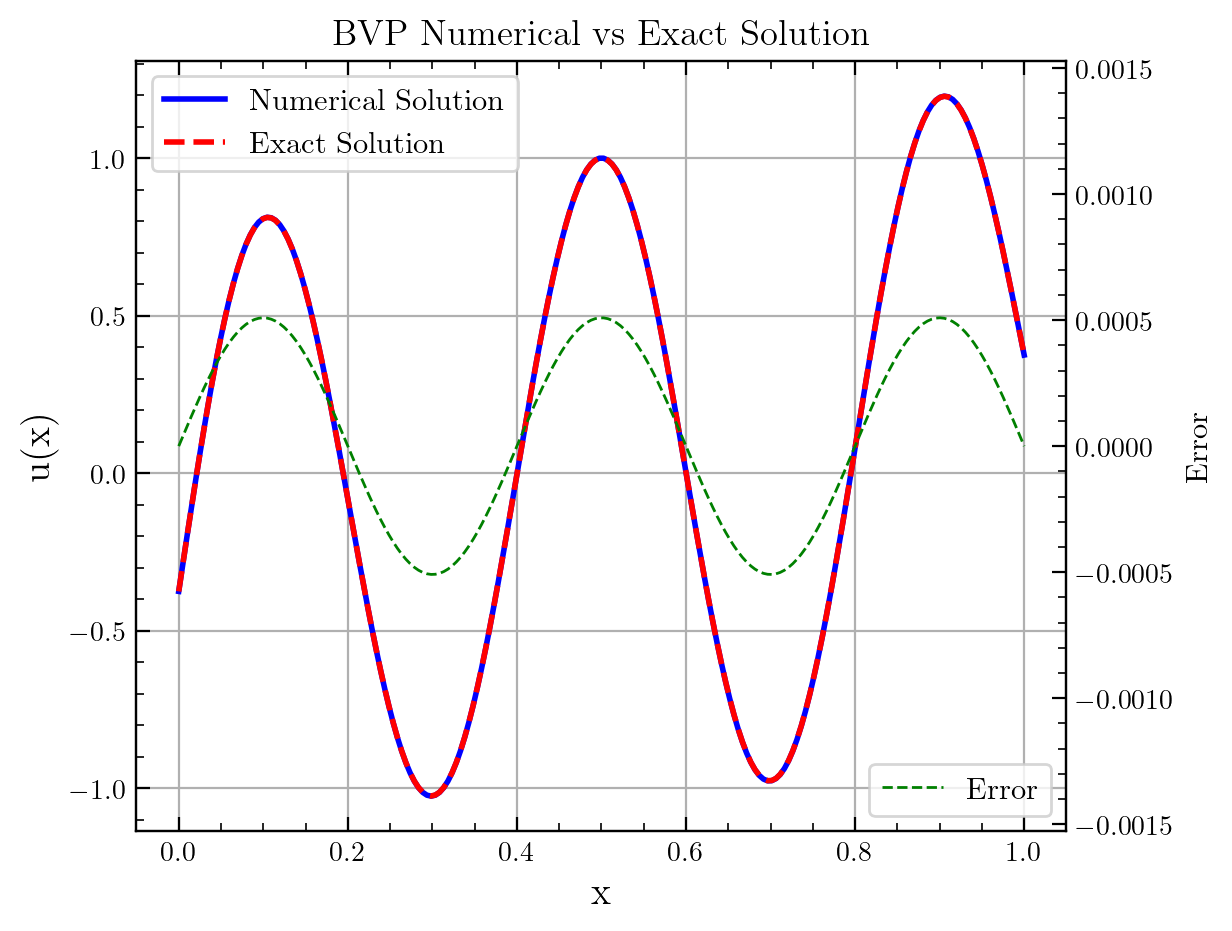
\includegraphics[width=1\textwidth] {../bvp_solution.png}
    \caption{The solution to the BVP with $k=5$, $\gamma=0$, and $c=3$.}
\end{figure*}

Now for the convergence study as a function of $h$, we can run the script
\begin{verbatim}
    run_3c.sh
\end{verbatim}
by either making it parallel (defaults to 4 processors) or not using the following targets
\begin{verbatim}
convergence:
	    chmod +x run_3c.sh
	    ./run_3c.sh

convergence_parallel:
	    chmod +x run_3c.sh
	    ./run_3c.sh 4
\end{verbatim}

And this gives us the following convergence plot, using the 4 processors (which is the same as the serial version also saved) which shows that the error decreases like $O(h^2)$ as expected for a second order finite difference method.
\begin{figure*}
   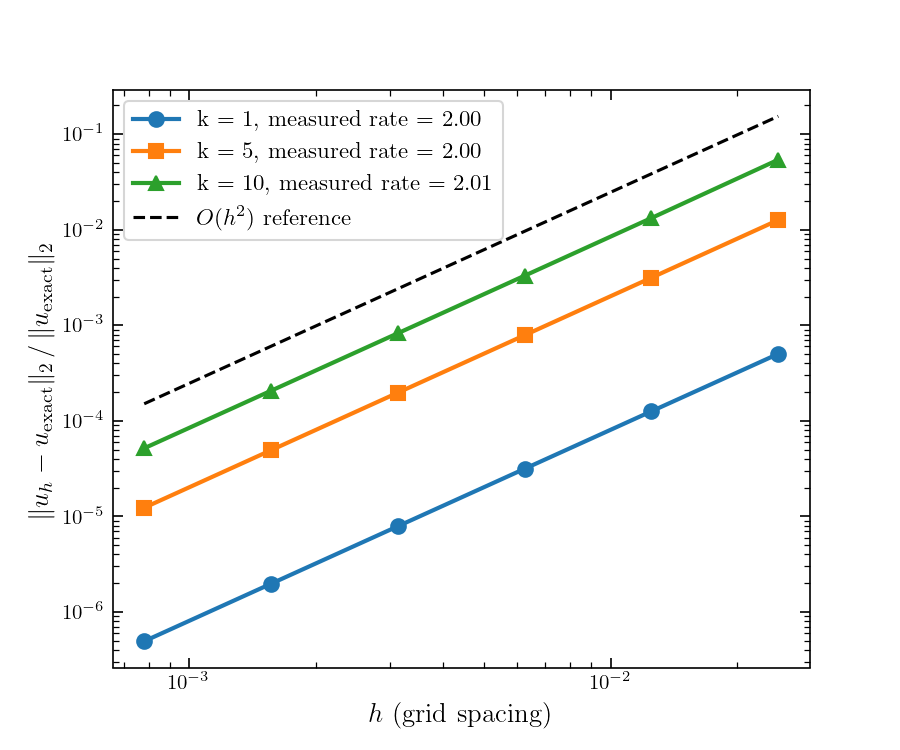
\includegraphics[width=1\textwidth] {../q3c_convergence_nP4.png}
    \caption{Convergence of the error as a function of $h$ -- using $m = 40, 80, 160, 320, 640, 1280$ --  for $k=1,5,10$ and $\gamma=0$.}
\end{figure*}

\section{Question 4, preconditioning}

all the results/ stdout are in 
\begin{verbatim}
    q4_stdouts
\end{verbatim} and the hdf5 files are in 
\begin{verbatim}
    bvp_hdf5_files.
\end{verbatim}

\subsection{part (a) jacobi pre-conditioned richardson}
We get the result
\begin{verbatim}
./bvp -options_file options_file -ksp_type richardson \ 
-pc_type jacobi -ksp_converged_reason -ksp_monitor  \ 

BVP: m=201  N=202  h=4.975124e-03  gamma=0.00  k=5.0  c=3.00
  0 KSP Residual norm 5.936478297702e-01
  1 KSP Residual norm 1.359022056691e-01
  2 KSP Residual norm 9.841291434704e-02
  3 KSP Residual norm 7.992980549991e-02
  4 KSP Residual norm 6.883656630639e-02
  5 KSP Residual norm 6.143186038119e-02
  6 KSP Residual norm 5.614321276949e-02
  ...
  10000 KSP Residual norm 1.723512279013e-04
  Linear solve did not converge due to DIVERGED_ITS iterations 10000
KSP converged reason: DIVERGED_ITS
m=201  h=4.975124e-03  ||u-uexact||/||uexact|| = 8.530933e-04
\end{verbatim}

From this we can see that we hit the maximum number of iterations (10,000) without convergence based on the tolerance we specify. Jacobi doesn really help it just divides each by its diagonal entry, which is not really doing much to help the convergence. 


\subsection{part (b) unconditioned conjugate gradient with 1 processor}
\begin{verbatim}
./bvp -options_file options_file \
-ksp_type cg -pc_type none \
-ksp_converged_reason -ksp_monitor \

BVP: m=201  N=202  h=4.975124e-03  gamma=0.00  k=5.0  c=3.00
  0 KSP Residual norm 2.155577866517e+04
  1 KSP Residual norm 1.111750882397e+04
  2 KSP Residual norm 7.998702608635e+03
  3 KSP Residual norm 6.834107103445e+03
  4 KSP Residual norm 6.537697820001e+03
  ...
  100 KSP Residual norm 1.978828404200e+01
  101 KSP Residual norm 5.068132641322e-01
  102 KSP Residual norm 3.765868642379e-05
  Linear solve converged due to CONVERGED_RTOL iterations 102
  KSP converged reason: CONVERGED_RTOL
  m=201  h=4.975124e-03  ||u-uexact||/||uexact|| = 4.988274e-04
\end{verbatim}

This one converges in 102 iterations, which is much better than the jacobi preconditioned richardson method, but still not great. By doing CG without preconditioning, we are still doing a lot of work to get the solution, and the convergence is not great. But, it is better than the jacobi preconditioned richardson method, which did not converge at all.


\subsection{part (c) unconditioned gradient with $c=0$}

\begin{verbatim}
./bvp -options_file options_file \
-bvp_c 0 -ksp_type cg -pc_type none \
-ksp_converged_reason -ksp_monitor \
BVP: m=201  N=202  h=4.975124e-03  gamma=0.00  k=5.0  c=0.00
  0 KSP Residual norm 2.473561911611e+03
  1 KSP Residual norm 8.897273067969e-09
  Linear solve converged due to CONVERGED_RTOL iterations 1
KSP converged reason: CONVERGED_RTOL
m=201  h=4.975124e-03  ||u-uexact||/||uexact|| = 5.090952e-04
\end{verbatim}

This is a special case where the solution is just a sine wave, and the finite difference discretization of the second derivative is exact for sine waves, so we get convergence in just 1 iteration.

\subsection{part (d) icc preconditioned conjugate gradient with 1 processors}
\begin{verbatim}
./bvp -options_file options_file \
-ksp_type cg -pc_type icc \
-ksp_converged_reason -ksp_monitor \

BVP: m=201  N=202  h=4.975124e-03  gamma=0.00  k=5.0  c=3.00
  0 KSP Residual norm 1.023632379439e+01
  1 KSP Residual norm 6.221130914797e-13
  Linear solve converged due to CONVERGED_ATOL iterations 1
KSP converged reason: CONVERGED_ATOL
m=201  h=4.975124e-03  ||u-uexact||/||uexact|| = 4.988274e-04
\end{verbatim}

This one is preconditioned with incomplete Cholesky factorization, which is a much better preconditioner than jacobi, and we get convergence in just 1 iteration,. The Cholesky faction of a tridiagonal matrix produces a tridiagonal matrix, it is exactly M = A, so the preconditioner is exact, and we get convergence in just 1 iteration.

\subsection{part (e) icc preconditioned conjugate gradient with 4 processors}

\begin{verbatim}
mpiexec -np 4 ./bvp -options_file options_file \
-ksp_type cg -pc_type bjacobi -sub_pc_type icc \
-ksp_converged_reason -ksp_monitor \

BVP: m=201  N=202  h=4.975124e-03  gamma=0.00  k=5.0  c=3.00
  0 KSP Residual norm 1.031869692986e+01
  1 KSP Residual norm 5.111556912929e-01
  2 KSP Residual norm 2.252222474944e-01
  3 KSP Residual norm 2.945416380291e-02
  4 KSP Residual norm 5.768915965017e-03
  5 KSP Residual norm 3.721823976221e-03
  6 KSP Residual norm 3.625002529575e-04
  7 KSP Residual norm 5.308486755828e-10
  Linear solve converged due to CONVERGED_RTOL iterations 7
KSP converged reason: CONVERGED_RTOL
m=201  h=4.975124e-03  ||u-uexact||/||uexact|| = 4.988273e-04
\end{verbatim}

Here, we pre condition with blocked Jacobi with 4 procesors, now each processer is doing an incomplete Cholesky factorization of a block of the matrix -- since it only sees its own chink of the matrix, the preconditioner is not exact, and we get convergence in 7 iterations, which is still pretty good, but not as good as the single processor version with exact incomplete Cholesky factorization. More processors means more boundary issues.

\subsection{part (f) direct solver}



with 1 processor
\begin{verbatim}
./bvp -options_file options_file \
-ksp_type preonly -pc_type lu \
-pc_factor_mat_solver_type mumps \
-ksp_converged_reason \

BVP: m=201  N=202  h=4.975124e-03  gamma=0.00  k=5.0  c=3.00
  0 KSP Residual norm 2.155577866517e+04
  1 KSP Residual norm 7.579263188166e-11
  Linear solve converged due to CONVERGED_ITS iterations 1
KSP converged reason: CONVERGED_ITS
m=201  h=4.975124e-03  ||u-uexact||/||uexact|| = 4.988274e-04
WARNING! There are options you set that were not used!
WARNING! could be spelling mistake, etc!
There are 2 unused database options. They are:
Option left: name:-ksp_atol value: 1.e-10 source: file
Option left: name:-ksp_rtol value: 1.e-8 source: file
\end{verbatim}

and 4 processors
\begin{verbatim}
BVP: m=201  N=202  h=4.975124e-03  gamma=0.00  k=5.0  c=3.00
  0 KSP Residual norm 2.155577866517e+04
  1 KSP Residual norm 7.523879334287e-11
  Linear solve converged due to CONVERGED_ITS iterations 1
KSP converged reason: CONVERGED_ITS
m=201  h=4.975124e-03  ||u-uexact||/||uexact|| = 4.988274e-04
WARNING! There are options you set that were not used!
WARNING! could be spelling mistake, etc!
There are 2 unused database options. They are:
Option left: name:-ksp_atol value: 1.e-10 source: file
Option left: name:-ksp_rtol value: 1.e-8 source: file

\end{verbatim}

Both of the runs above is a direct solve with no preconditioner. This does not differ between processors because the direct solver is not parallelized in any way, so it is the same regardless of how many processors are used. MUMPS does not iterate at all since it just compute the exact factorication of A and applies it. Floating point errors can cause the residual to be nonzero, but it is very small, and we get convergence in just 1 iteration. 
The warning about the unused options is just because we are using the same options file for all the runs, and some of the options we specify in the options file are not used for the direct solve, since it does not iterate at all and does not check tolerences, so it just ignores those options.

\end{document}